\documentclass{standalone}
\usepackage{tikz, ifthen}
\usepackage{amsmath}

\begin{document}

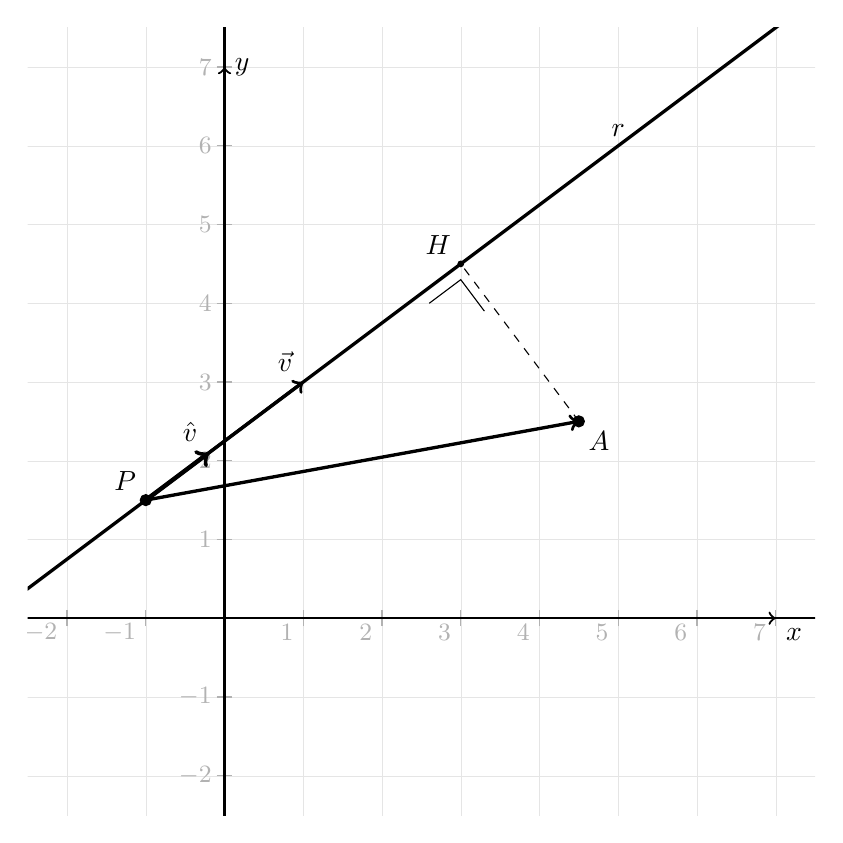
\begin{tikzpicture}
    
    % Center of the circle
    \def\xmin{-2}
    \def\xmax{7}
    \def\ymin{-2}
    \def\ymax{7}
    \def\dx{.5}
    \def\dy{.5}
    \def\xminb{\xmin-\dx}
    \def\xmaxb{\xmax+\dx}
    \def\yminb{\ymin-\dy}
    \def\ymaxb{\ymax+\dy}
    \def\xa{4.5}     % xA
    \def\ya{2.5}     % yA
    \def\xb{3  }     % xB
    \def\yb{4.5}     % yB
    \def\xpmin{-6}
    \def\xpmax{ 6}
    \def\ypmin{-5.5}
    \def\ypmax{ 5.5}
%   \def\a{0.5};
%   \coordinate (fa) at (\xa, \ya);
%   \coordinate (fb) at (\xb, \yb);
%   \def\c{sqrt((\xa-\xb)^2+(\ya-\yb)^2)/2};
%   \def\xc{0.5*(\xa+\xb)};
%   \def\yc{0.5*(\ya+\yb)};
%   \coordinate (center) at ({\xc}, {\yc});
%   \def\b{sqrt(\c^2-\a^2)};
%   \def\alpha{{atan2(\yb-\ya,\xb-\xa)}};

    \clip (\xminb, \yminb) rectangle (\xmaxb, \ymaxb);

    % Draw grid
    \draw[step=1., gray!20, ultra thin] (\xmin-2, \ymin-2) grid (\xmax+2, \ymax+2); % Visible grid with lighter color

    % Axis ticks
    \foreach \x in {\xmin,..., \xmax}{
        \ifthenelse{ \x = 0 }{}{\draw[black!30] (\x, -0.1) -- (\x, +0.1) node[below=8pt, left=0pt] {\small $\x$};}
    }
    \foreach \y in {\ymin,..., \ymax}{
        \ifthenelse{ \y = 0 }{}{\draw[black!30] (-0.1, \y) -- (0.1, \y) node[left=4pt] {\small $\y$};}
    }
    % Axes, x
    \draw[->, thick, black] (\xmin, 0) -- (\xmax, 0) node[below right] {$x$};
    \draw[->, thick, black] (0, \ymin) -- (0, \ymax) node[right] {$y$};
    \draw[    thick, black] (\xmin-2, 0) -- (\xmax+2, 0);
    \draw[    thick, black] (0, \ymin-2) -- (0, \ymax+2);

    \draw[very thick, black] (-3,0) -- (9,9);
    \filldraw[black] (5,6) circle (0pt) node[above] {$r$};
    \draw[black] (3-0.4,4.5-0.5) -- (3,4.5-.2) -- (3+.3,4.5-.6);
    \filldraw[black] (\xb,\yb) circle (1pt) node[above left] {$H$};
    \draw[black, dashed] (\xa,\ya) -- (\xb,\yb);
    \filldraw[black] (\xa,\ya) circle (2pt) node[below right] {$A$}; % \equiv (x_A, y_A)$};
    \filldraw[black] (-1, 1.5) circle (2pt) node[above left ] {$P$}; % \equiv (x_A, y_A)$};
    \draw[->, black, very thick] (-1,1.5) -- (\xa,\ya);
    \draw[->, black, very thick] (-1,1.5) -- (1,3) node[above left] {$\vec{v}$};
    \draw[->, black, ultra thick] (-1,1.5) -- (-0.2, 2.1) node[above left] {$\hat{v}$};


%   \draw[black, dashed, ] (0,\ya) node[left ] {$y_A$} -- (\xb+.5, \ya);
%   \draw[black, dashed, ] (0,\yb) node[left ] {$y_B$} -- (\xb+.5, \yb);
%   \draw[black, dashed, ] (\xa,0) node[below left] {$x_A$} -- (\xa, \yb);
%   \draw[black, dashed, ] (\xb,0) node[below left] {$x_B$} -- (\xb, \yb);
%   \draw[black, dashed, ] (\xa,\ya) -- (\xb, \yb);

%   \draw[<->, thick, black] (\xa,2.5) -- (\xb,2.5) node[midway, below] {$|x_B-x_A|$};
%   \draw[<->, thick, black] (5.5,\ya) -- (5.5,\yb) node[midway, below, rotate=90] {$|y_B-y_A|$};
%   \draw[<->, thick, black] (\xa-0.3,\ya+0.4) -- (\xb-0.3,\yb+0.4) node[midway, above, rotate=36.8] {$\text{dist}(A,B)$};

%   % Origin
%   \filldraw[black] (0,0) circle (2pt) node[below left] {$O$};

%   \filldraw[black] (\xa,\ya) circle (2pt) node[below left ] {$A$}; % \equiv (x_A, y_A)$};
%   \filldraw[black] (\xb,\yb) circle (2pt) node[above right] {$B$}; % \equiv (x_B, y_B)$};


%   % Foci
%   \filldraw[black] (\xa, \ya) circle (2pt) node[above right] {$0$};
%   \filldraw[black] (\xb, \yb) circle (2pt) node[above right] {$2$};
    
\end{tikzpicture}

\end{document}
